\documentclass{article}
\usepackage{tikz}
\usetikzlibrary{arrows.meta, positioning}

\begin{document}

\begin{figure}[ht]
\centering  
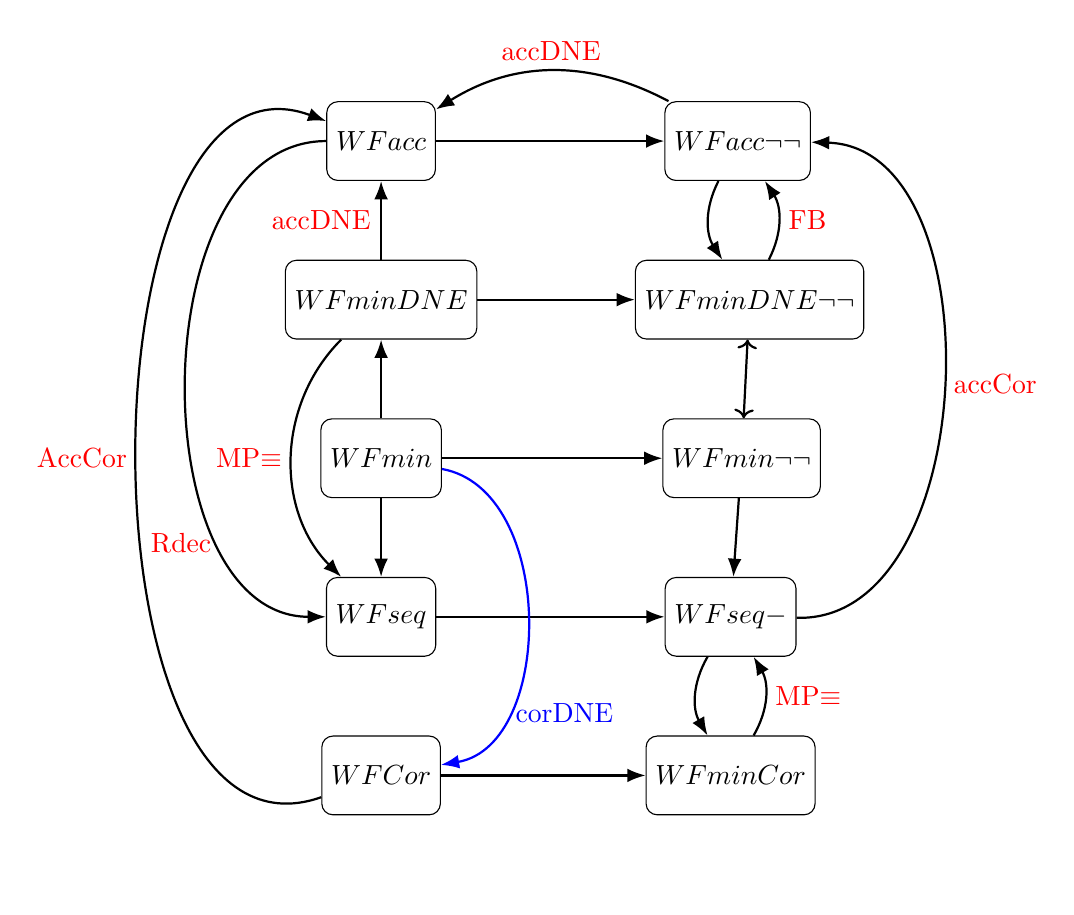
\begin{tikzpicture}[
  node distance=1cm and .5cm,
  box/.style={draw, rectangle, rounded corners, minimum width=1cm, minimum height=1cm, align=center},
  arrow/.style={-{Latex}, thick}
]

% Row 1: WFacc
\node[box] (WFacc) {$WFacc$};
% \node[box, right=of WFacc] (NNWFacc) {$\lnot\lnot$WFacc};
\node[box, right=2.9cm of WFacc] (WFaccM) {$WFacc\lnot\lnot$};

\draw[arrow] (WFacc) -- (WFaccM);
% \draw[arrow] (NNWFacc) -- (WFaccM);
\draw[arrow, bend right] (WFaccM) to node[above, text=red] {accDNE} (WFacc);

% Row 2: WFind
% \node[box, below=of WFacc] (WFind) {WFind};
% \node[box, right=of WFind] (NNWFind) {$\lnot\lnot$WFind};
% \node[box, right=of NNWFind] (WFindM) {WFind-};

% \draw[arrow] (WFind) -- (NNWFind);
% \draw[arrow] (NNWFind) -- (WFindM);


% \draw[arrow] (NNWFseq) -- (WFseqM);

% Row 5: WFminDNE -> WFminDNE-
\node[box, below=of WFacc] (WFminDNE) {$WFminDNE$};
\node[box, right=2.0cm of WFminDNE] (WFminDNEM) {$WFminDNE\lnot\lnot$};

\draw[arrow] (WFminDNE) -- (WFminDNEM);

% Row 4: WFmin -> WFmin-
\node[box, below=of WFminDNE] (WFmin) {$WFmin$};
\node[box, right=2.8cm of WFmin] (WFminM) {$WFmin\lnot\lnot$};

\draw[arrow] (WFmin) -- (WFminM);



% Row 3: WFseq
\node[box, below=of WFmin] (WFseq) {$WFseq$};
% \node[box, right=of WFseq] (NNWFseq) {$\lnot\lnot$WFseq};
\node[box, right=2.9cm of WFseq] (WFseqM) {$WFseq-$};

\draw[arrow] (WFseq) -- (WFseqM);

% Row 6: WFcor 
\node[box, below=of WFseq] (WFCor) {$WFCor$};
\node[box, below=of WFseqM] (WFminCor) {$WFminCor$};


% Arrows between rows
% \draw[arrow, <->] (WFacc) -- (WFind);
% \draw[arrow, <->] (NNWFacc) -- (NNWFind);
% \draw[arrow, <->] (WFaccM) -- (WFindM);

\draw[arrow, bend right = 90] (WFacc) to node[pos = 0.75,left, text = red] {Rdec} (WFseq);
\draw[arrow, bend right] (WFaccM) to (WFminDNEM);
\draw[arrow, bend right = 90] (WFseqM) to node[right, text=red] {accCor} (WFaccM);  
% \draw[arrow, bend left = 55] (WFaccM) to (WFminM);  


\draw[arrow] (WFmin) -- (WFseq);
\draw[arrow] (WFminM) -- (WFseqM);
\draw[arrow] (WFmin) -- (WFminDNE);
\draw[arrow, <->] (WFminM) -- (WFminDNEM);

\draw[arrow] (WFminDNE) to node[left, text = red] {accDNE} (WFacc);
\draw[arrow, bend right=45] (WFminDNE) to node[pos=0.5, left, text=red] {MP$\equiv$} (WFseq);
\draw[arrow, bend right] (WFminDNEM) to node[right, text=red] {FB} (WFaccM);
\draw[arrow, bend right] (WFseqM) to (WFminCor);
\draw[arrow, bend right] (WFminCor) to node [right, text=red] {MP$\equiv$} (WFseqM);
\draw[arrow] (WFCor) -- (WFminCor);
\draw[arrow, bend left = 110] (WFCor) to node[left, text=red] {AccCor} (WFacc);
\draw[arrow, bend left = 80, color=blue] (WFmin) to node[right, text=blue, pos=0.75] {corDNE} (WFCor);
 

\end{tikzpicture}
\caption{The logical relationships between notions of well-foundedness}
 \label{fig:WF} 
\end{figure}
\clearpage

\end{document}
